\documentclass[xcolor=dvipsnames]{beamer}

\usetheme{AnnArbor}
\usepackage{dsfont}
\usepackage{amsmath}
\usepackage{caption}
\usepackage{hyperref}
\usepackage{xcolor}
\usepackage{color}
\usepackage{commath}
\usepackage{physics}
\usepackage{enumerate}
\usepackage{hyperref}
\usepackage{graphics}
\usepackage{subcaption}

%\usepackage[backend=bibtex, style=authoryear-comp]{biblatex}

\setbeamertemplate{bibliography item}{\insertbiblabel}
\beamertemplatenavigationsymbolsempty

\usepackage{filecontents}
\begin{filecontents}{\jobname.bib}
@incollection{aldous1985exchangeability,
  title={Exchangeability and related topics},
  author={Aldous, David J},
  booktitle={{\'E}cole d'{\'E}t{\'e} de Probabilit{\'e}s de Saint-Flour XIII—1983},
  pages={1--198},
  year={1985},
  publisher={Springer}
}
@Article{quanteda,
  title = {quanteda: An R package for the quantitative analysis of textual data},
  journal = {Journal of Open Source Software},
  author = {Kenneth Benoit and Kohei Watanabe and Haiyan Wang and Paul Nulty and Adam Obeng and Stefan Müller and Akitaka Matsuo},
  doi = {10.21105/joss.00774},
  url = {https://quanteda.io},
  volume = {3},
  number = {30},
  pages = {774},
  year = {2018},
}
@article{blei2012probabilistic,
  title={Probabilistic topic models},
  author={Blei, David M},
  journal={Communications of the ACM},
  volume={55},
  number={4},
  pages={77--84},
  year={2012},
  publisher={ACM New York, NY, USA}
}
@article{blei2003latent,
  title={Latent dirichlet allocation},
  author={Blei, David M and Ng, Andrew Y and Jordan, Michael I},
  journal={Journal of machine Learning research},
  volume={3},
  number={Jan},
  pages={993--1022},
  year={2003}
}
@article{lucas2015computer,
  title={Computer-assisted text analysis for comparative politics},
  author={Lucas, Christopher and Nielsen, Richard A and Roberts, Margaret E and Stewart, Brandon M and Storer, Alex and Tingley, Dustin},
  journal={Political Analysis},
  volume={23},
  number={2},
  pages={254--277},
  year={2015},
  publisher={Cambridge University Press}
}
@Manual{R,
  title        = {R: A Language and Environment for Statistical Computing},
  author       = {{R Core Team}},
  organization = {R Foundation for Statistical Computing},
  address      = {Vienna, Austria},
  year         = 2020,
  url          = {https://www.R-project.org}
}
@article{richardson2007beautiful,
  title={Beautiful soup documentation},
  author={Richardson, Leonard},
  journal={April},
  year={2007}
}
@article{roberts2016model,
  title={A model of text for experimentation in the social sciences},
  author={Margaret E. Roberts and Brandon M. Stewart and Edoardo M. Airoldi},
  journal={Journal of the American Statistical Association},
  volume={111},
  number={515},
  pages={988--1003},
  year={2016},
  publisher={Taylor \& Francis}
}
@article{roesslein2020tweepy,
  title={Tweepy: Twitter for Python!},
  author={Roesslein, Joshua},
  journal={URL: https://github.com/tweepy/tweepy},
  year={2020}
}
@book{van1995python,
  title={Python reference manual},
  author={Van Rossum, Guido and Drake Jr, Fred L},
  year={1995},
  publisher={Centrum voor Wiskunde en Informatica Amsterdam}
}
\end{filecontents}
\usepackage[style=authoryear]{biblatex}
\renewcommand*{\nameyeardelim}{\addcomma\addspace}
\addbibresource{\jobname.bib}

\newcommand{\customcite}[1]{\citeauthor{#1} (\citeyear{#1})}

\newtheorem{satz}{Satz}

\setbeamertemplate{footline}[page number]

\usecolortheme{seagull}
\setbeamercolor{frametitle}{fg=blue,bg=White}

%\DeclareMathOperator*{\argmax}{arg\, max}
%\DeclareMathOperator*{\argmin}{arg\, min}
%\setbeamertemplate{section in toc}[sections numbered]
%\setbeamertemplate{subsection in toc}[subsections numbered]
%\AtBeginSection[]
%{
%\begin{frame}
%\frametitle{Überblick}
%\tableofcontents[currentsection]
%\end{frame}
%}
%
%\AtBeginSubsection[
% {\frame<beamer>{\frametitle{Überblick}   
%  \tableofcontents[currentsection,currentsubsection]}}%
%]%
%{
 % \frame<beamer>{ 
 %   \frametitle{Überblick}   
   % \tableofcontents[currentsection,currentsubsection]}
%}

\title{Twitter in the Parliament - A Text-based Analysis of German Political Entities}
%\author{Patrick Schulze}
\date{7. Juli 2020}
\author[author1]{Patrick Schulze, Simon Wiegrebe\\[10mm]{\small Supervisors:\\ Prof. Dr. Christian Heumann, Prof. Dr. Paul W. Thurner}}

\begin{document}

\begin{frame}
\titlepage
\end{frame}

%\begin{frame}
%\frametitle{Überblick}
%\tableofcontents[]
%\end{frame}

\section{Introduction}
\begin{frame}
\frametitle{Introduction}
\begin{itemize}
\item Huge amounts of data, especially text, produced by social media
\item Field of particular interest in the context of social media and big data: \textit{Politics} (e.g., Brexit, 2016 presidential election in the US, Facebook data scandal).
\item Tools of analysis for such data simultaneously provided by advances in \textit{Natural Language Processing} (NLP)
\item \textit{topic analysis}: analytical tool for discovery and exploration of latent thematic clusters within text
\item In this project: application of the \textit{Structural Topic Model} (STM) \cite{roberts2016model} to a self-created dataset containing Twitter posts by members of the German Bundestag (and a variety of metadata) 
\end{itemize}
\end{frame}

\section{Topic Modeling: Motivation and Theory}
\begin{frame}
\frametitle{Topic Modeling: Motivation and Theory}
\framesubtitle{Notation and Terminology (I)}
\begin{itemize}
\item \textit{Words} $w$: instances of a vocabulary of $V$ unique \textit{terms}.
\item \textit{Documents} $d \in \{1,\dots,D\}$: sequences of words of length $N_{d}$; $w_{d,n}$ denoting $n$-th word of document $d$
\item \textit{Corpus}: collection (or set) of $D$ documents
\item \textit{Topics} $k \in \{1,\dots,K\}$: latent thematic clusters within a text corpus; (implicit) representation of a corpus
\item \textit{Topic-word distributions} $\boldsymbol{\beta}$: probability distributions over words; $\boldsymbol{\beta}_k$ denoting the word distribution corresponding to the $k$-th topic
\end{itemize}
\end{frame}

\begin{frame}
\frametitle{Topic Modeling: Motivation and Theory}
\framesubtitle{Notation and Terminology (II)}
\begin{itemize}
\item \textit{Topic assignments} $\boldsymbol{z}_{d,n}$: assignment of $w_{d,n}$ to a specific topic $k \in \{1,\dots,K\}$; $\boldsymbol{\beta}_{d,n}$ representing the (assigned) word distribution for $w_{d,n}$
\item \textit{Topic proportions} $\boldsymbol{\theta}_d$: proportions of document $d$'s terms assigned to each of the topics; $\sum_{k=1}^{K}\theta_{d,k}=1$, for all $d \in \{1,\dots,D\}$
\item \textit{Bag-of-word} assumption: only words themselves meaningful, unlike word order or grammar; equivalent to assuming \textit{exchangeability} \cite{aldous1985exchangeability}.
\end{itemize}
\end{frame}

\begin{frame}
\frametitle{Topic Modeling: Motivation and Theory}
\framesubtitle{\textit{Latent Dirichlet Allocation} (LDA) (I)}
\begin{itemize}
\item First topic model with entirely probabilistic generating process: LDA \cite{blei2003latent}
\item Generative process for each document $d \in \{1,\dots,D\}$:
\item[] 
	\begin{enumerate}[{1)}]
	\item Draw topic proportions $\boldsymbol{\theta}_d \sim \text{Dir}_K(\boldsymbol{\alpha})$.
	\item For each word $n \in \{1,\dots,N_d\}$:
		\begin{enumerate}[{a)}]
		\item Draw a topic assignment $\boldsymbol{z_{d,n}} \sim \text{Multinomial}_K(\boldsymbol{\theta}_d)$.
		\item Draw a word $w_{d,n} \sim \text{Multinomial}_V(\boldsymbol{\beta}_{d,n})$.
	\end{enumerate}
\end{enumerate}
\item Graphical model representation of LDA: \cite{blei2003latent} 
	\begin{figure}[h!]
  	\centering
  	\hspace*{-1cm}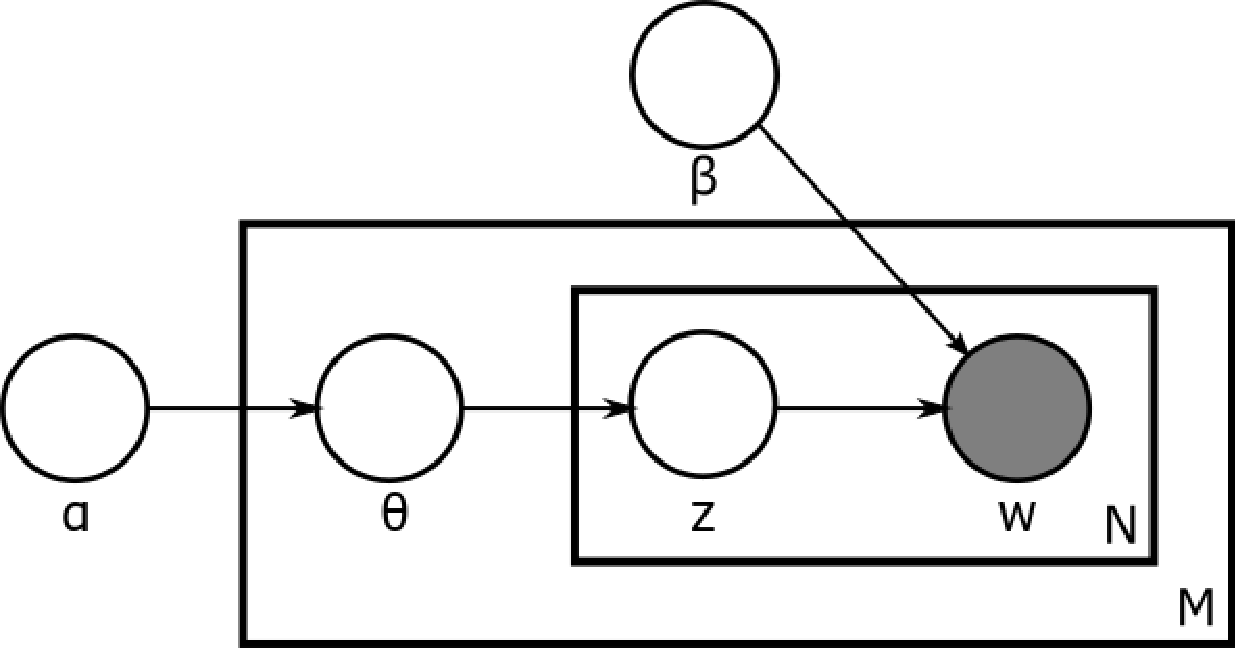
\includegraphics[scale = 0.3]{../plots/presentation/lda_graphical.pdf}
	\end{figure}
\end{itemize}
\end{frame}

\begin{frame}
\frametitle{Topic Modeling: Motivation and Theory}
\framesubtitle{\textit{Latent Dirichlet Allocation} (LDA) (II)}
\begin{itemize}
\vspace{-0.5cm}
\item Illustration of topic assignment for the words of a document: \cite{blei2012probabilistic}
	\vspace{-0.5cm}
	\begin{figure}[h!]
  	\centering
  	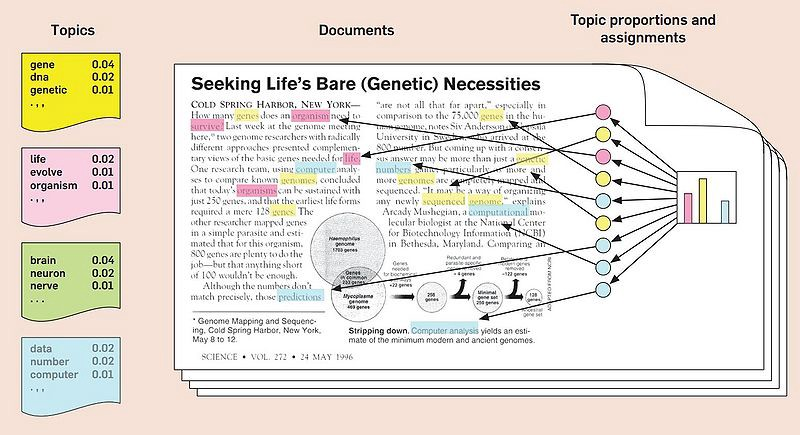
\includegraphics[scale = 0.4]{../plots/presentation/lda_topic_assignment.jpeg}
	\end{figure}
\end{itemize}
\end{frame}

\section{Data}
\begin{frame}
\frametitle{Data}
\framesubtitle{Data Collection (I)}
\begin{itemize}
\item MP-level data: from \url{www.bundestag.de/abgeordnete} using Python's \textit{BeautifulSoup} and a \textit{selenium web driver} \cite{van1995python} \cite{richardson2007beautiful}
\item[] 
	\begin{figure}[h!]
  	\centering
  	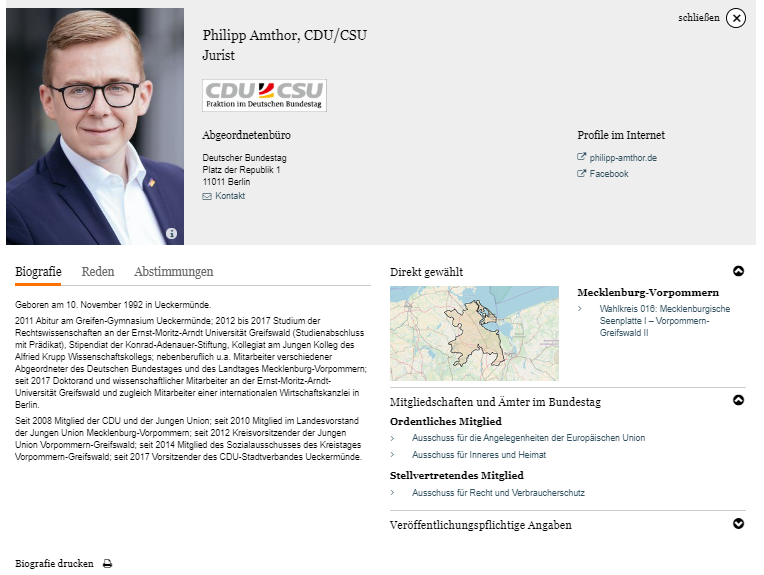
\includegraphics[scale = 0.42]{../plots/presentation/amthor.png}
	\end{figure}
\item Twitter profiles: from official party homepages
\item Socioeconomic data and 2017 German federal election results: from \url{www.bundeswahlleiter.de}.
\end{itemize}
\end{frame}

\begin{frame}
\frametitle{Data}
\framesubtitle{Data Collection (II)}
\begin{itemize}
\item Tweets (and further Twitter features): via the official Twitter API using Python's \textit{tweepy} library\cite{roesslein2020tweepy}
\item Monthly tweets (after dropping MPs without electoral district) for our period of analysis, September 24, 2017 through April 24, 2020:
	\begin{figure}[h!]
  	\centering
  	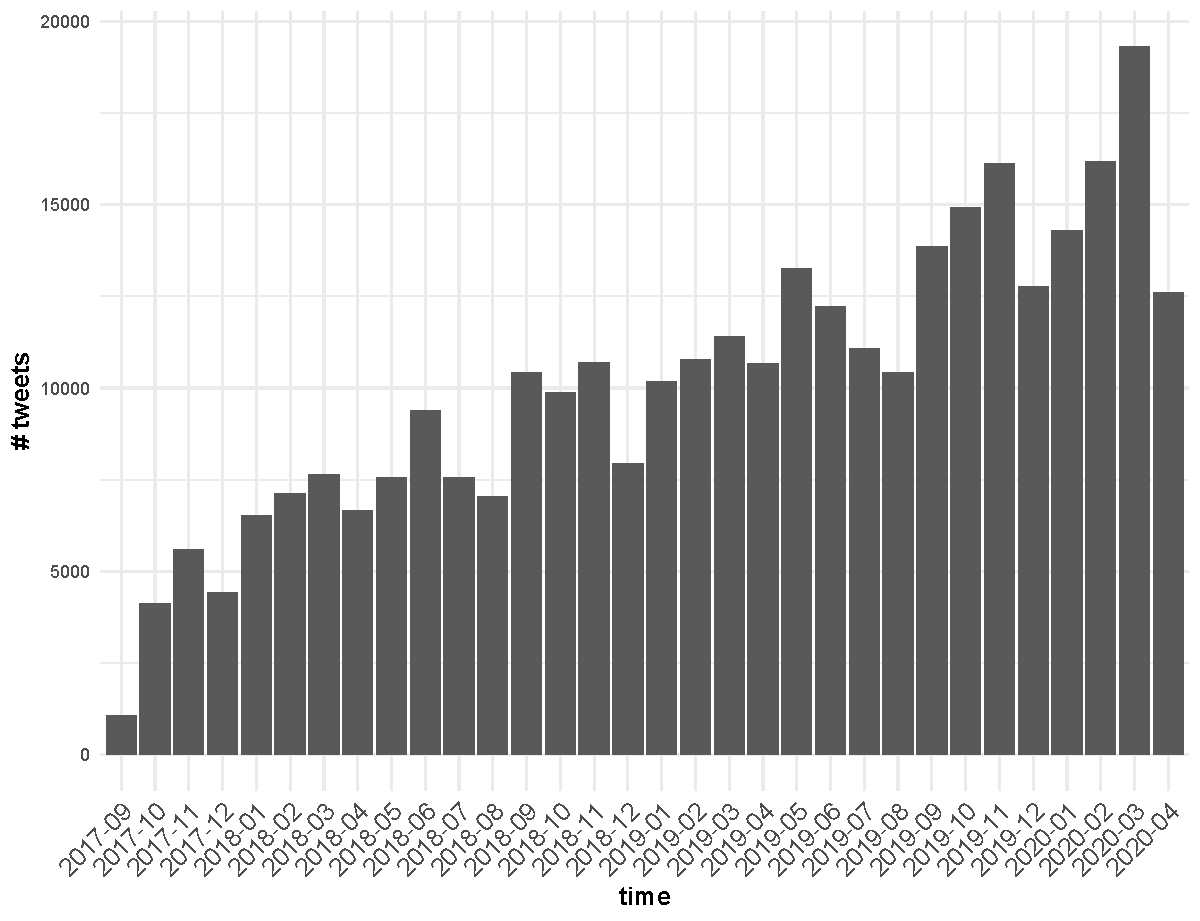
\includegraphics[scale = 0.30]{../plots/3/monthly_tweets.pdf}
	\end{figure}
\item In the following: grouping each MP's tweets on a monthly basis
\end{itemize}
\end{frame}

\begin{frame}
\frametitle{Data}
\framesubtitle{Data Preprocessing}
\begin{itemize}
\item Preprocessing: in R \cite{R}, using the \textit{quanteda} package \cite{quanteda}
\item Transcription of German umlauts (\"a/\"A, \"o/\"O, \"u/\"U) and ligature (\ss)
\item Removal of hyphens: relevant for compound words (e.g., \textit{Corona-Krise} vs \textit{Coronakrise})
\item Transformation of text data into document-feature matrix (DFM); conversion to lowercase; removal of stopword, units (\textit{kg}, \textit{uhr}), interjections (\textit{aaahhh}, \textit{ufff}), etc.
\item Word stemming, i.e., cutting off word endings (e.g., \textit{politisch} $\rightarrow$ \textit{polit}) \cite{lucas2015computer}
\end{itemize}
\end{frame}

\section{Model Selection and Global Characteristics}
\begin{frame}
\frametitle{Model Selection and Global Characteristics}
\framesubtitle{Model Selection}
\begin{itemize}
\item Model evaluation metrics for hyperparameter $K$ (number of topics):
	\begin{figure}[h!]
  	\centering
  	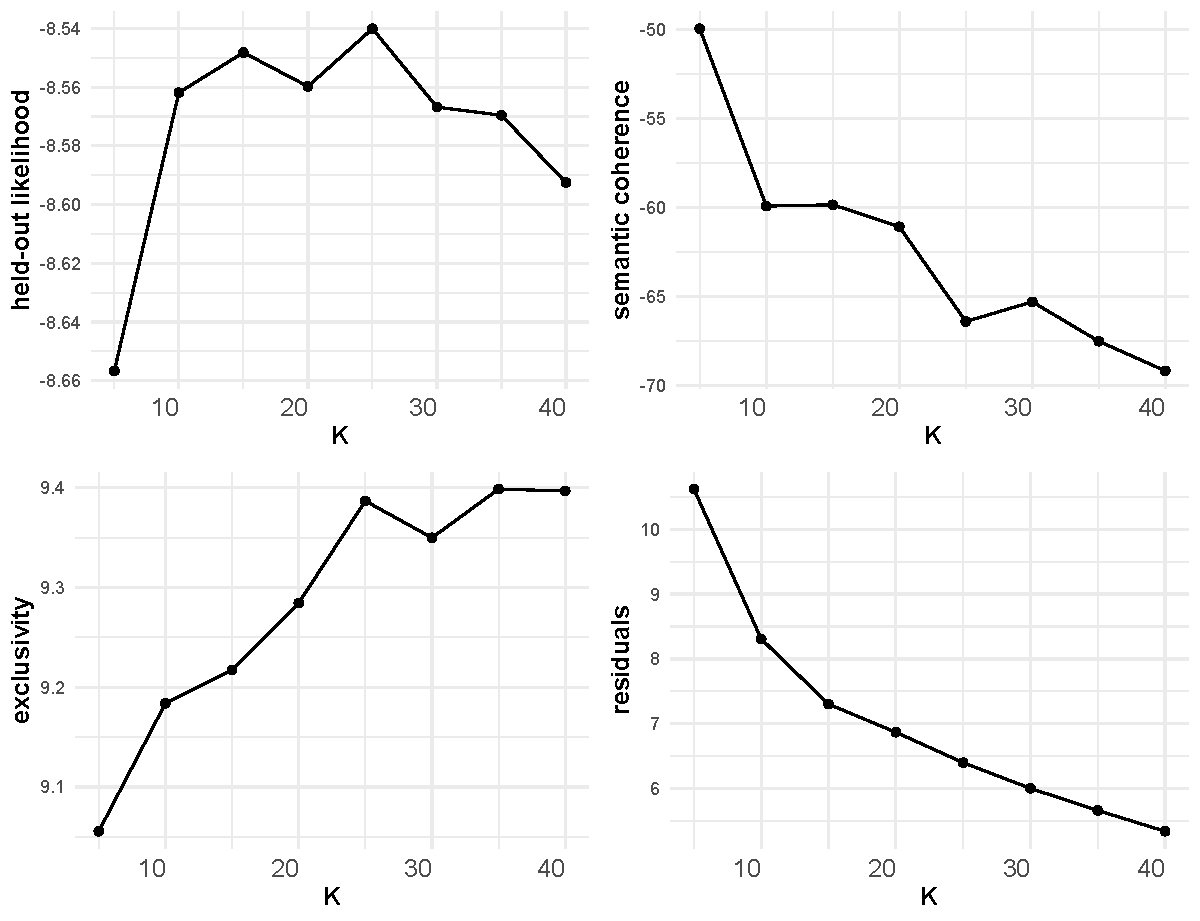
\includegraphics[scale = 0.30]{../plots/4_1/searchK.pdf}
	\end{figure}
\item Best trade-off: $K=15$
\end{itemize}
\end{frame}

\begin{frame}
\frametitle{Model Selection and Global Characteristics}
\framesubtitle{Labeling (I)}
\begin{itemize}
\item Three-step procedure for labeling
\item First step: top words for different weighting methodologies
\begin{table}[h!]
\centering
\resizebox{8cm}{!}{%
\begin{tabular}{|l|}
\hline
\textit{Topic 1 Top Words:}\\
 	 \textbf{Highest Prob:} buerg, link, merkel, frau, sich \\
 	 \textbf{FREX:} altpartei, islam, linksextremist, asylbewerb, linksextrem \\
 	 \textbf{Lift:} eitan, 22jaehrig, abdelsamad, abgehalftert, afdforder \\
 	 \textbf{Score:} altpartei, linksextremist, frauenkongress, islamist, boehring \\
\hline
\textit{Topic 3 Top Words:}\\
 	 \textbf{Highest Prob:} brauch, wichtig, leid, dank, klar \\
 	 \textbf{FREX:} emissionshandel, soli, marktwirtschaft, feedback, co2steu \\
 	 \textbf{Lift:} aequivalenz, altersvorsorgeprodukt, bildungsqualitaet, co2limit, co2meng \\
 	 \textbf{Score:} emissionshandel, co2limit, basisrent, euet, technologieoff \\
\hline
\textit{Topic 4 Top Words:}\\
 	 \textbf{Highest Prob:} sozial, miet, kind, arbeit, brauch \\
 	 \textbf{FREX:} mindestlohn, miet, wohnungsbau, mieterinn, loehn \\
 	 \textbf{Lift:} auseinanderfaellt, baugipfel, bestandsmiet, billigflieg, binnennachfrag \\
 	 \textbf{Score:} miet, mieterinn, mietendeckel, grundsicher, bezahlbar \\
\hline
\textit{Topic 6 Top Words:}\\
 	 \textbf{Highest Prob:} gruen, klimaschutz, brauch, klar, euro \\
 	 \textbf{FREX:} fossil, erneuerbar, kohleausstieg, verkehrsminist, verkehrsw \\
 	 \textbf{Lift:} abgasbetrug, abgebaggert, abschalteinricht, abschaltet, ammoniak \\ 
 	 \textbf{Score:} erneuerbar, fossil, zdebel, verkehrsminist, klimaschutz \\
\hline
\end{tabular}%
}
\end{table}
\end{itemize}
\end{frame}

\begin{frame}
\frametitle{Model Selection and Global Characteristics}
\framesubtitle{Labeling (II)}
\begin{itemize}
\item Word cloud of \textbf{Highest Prob} top words (for topic 1):
	\begin{figure}[h!]
  	\centering
  	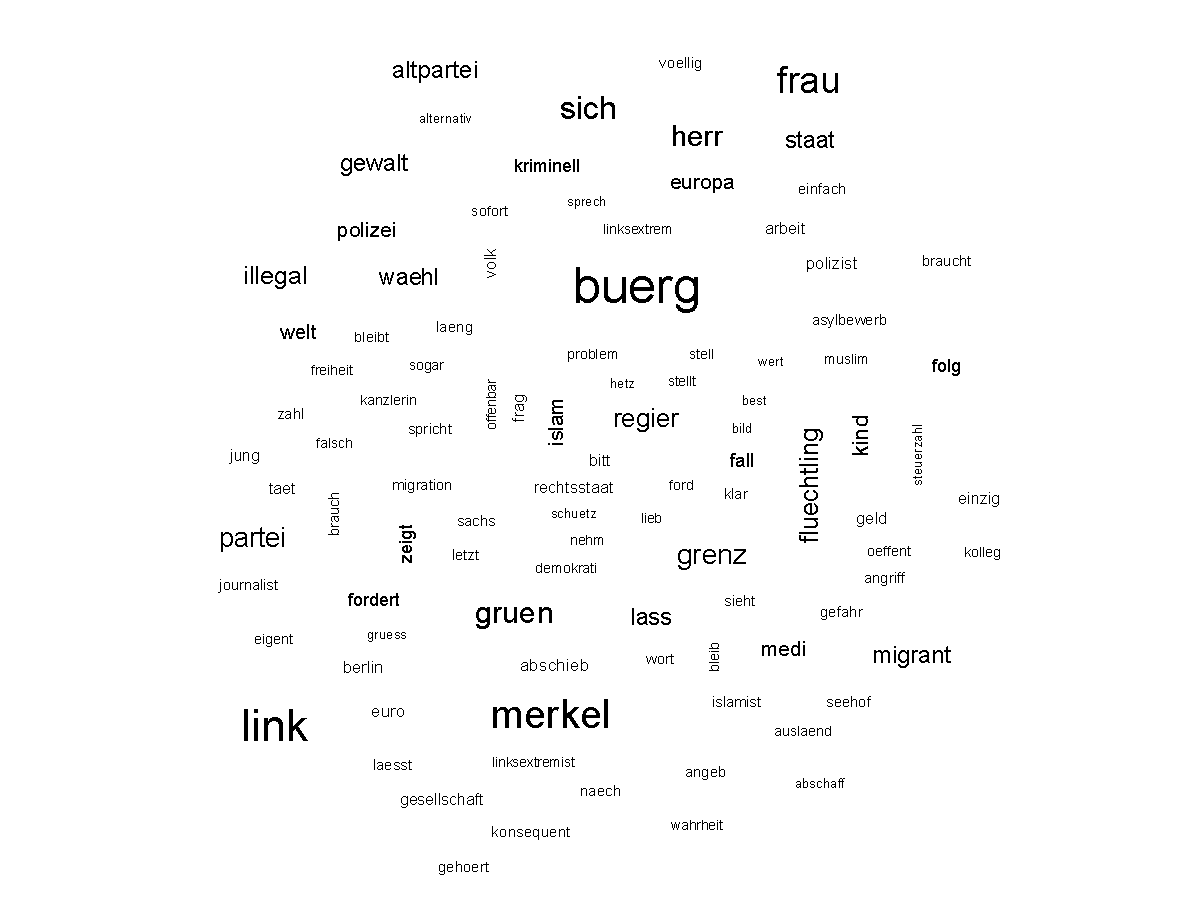
\includegraphics[scale = 0.40]{../plots/4_2/t1_wordcloud.pdf}
	\end{figure}
\item Word size corresponding to word frequency in topic 1
\end{itemize}
\end{frame}

\begin{frame}
\frametitle{Model Selection and Global Characteristics}
\framesubtitle{Labeling (III)}
\begin{itemize}
\item Second step: look at documents (i.e., original tweets) with highest proportion of topic 1
	\begin{figure}[h!]
  	\centering
  	
\includegraphics[scale = 0.40]{../plots/presentation/martin_hess_topic1.png}
	\end{figure}
\end{itemize}
\end{frame}

\begin{frame}
\frametitle{Model Selection and Global Characteristics}
\framesubtitle{Labeling (IV)}
\begin{itemize}
\item Third step: assigning labels
\begin{table}[h!]
	\centering
	\resizebox{5cm}{!}{%
	\begin{tabular}{|l|l|}
	\hline
	Topic 1  & Right/Nationalist    \\ \hline
	Topic 2  & Miscellaneous 1      \\ \hline
	Topic 3  & Climate Economics    \\ \hline
	Topic 4  & Social/Housing       \\ \hline
	Topic 5  & Digital/Future       \\ \hline
	Topic 6  & Climate Protection   \\ \hline
	Topic 7  & Europe               \\ \hline
	Topic 8  & Corona               \\ \hline
	Topic 9  & Left/Anti-war        \\ \hline
	Topic 10 & Twitter/Politics 1   \\ \hline
	Topic 11 & Twitter/Politics 2   \\ \hline
	Topic 12 & Miscellaneous 2      \\ \hline
	Topic 13 & Twitter/Politics 3   \\ \hline
	Topic 14 & Right-wing Extremism \\ \hline
	Topic 15 & Society/Solidarity   \\ \hline
	\end{tabular}
	}
\end{table}
\end{itemize}
\end{frame}

\begin{frame}
\frametitle{Model Selection and Global Characteristics}
\framesubtitle{Global Topic Proportions}
\begin{itemize}
\item Illustration of \textbf{global} topic proportions:
	\begin{figure}[h!]
  	\centering
  	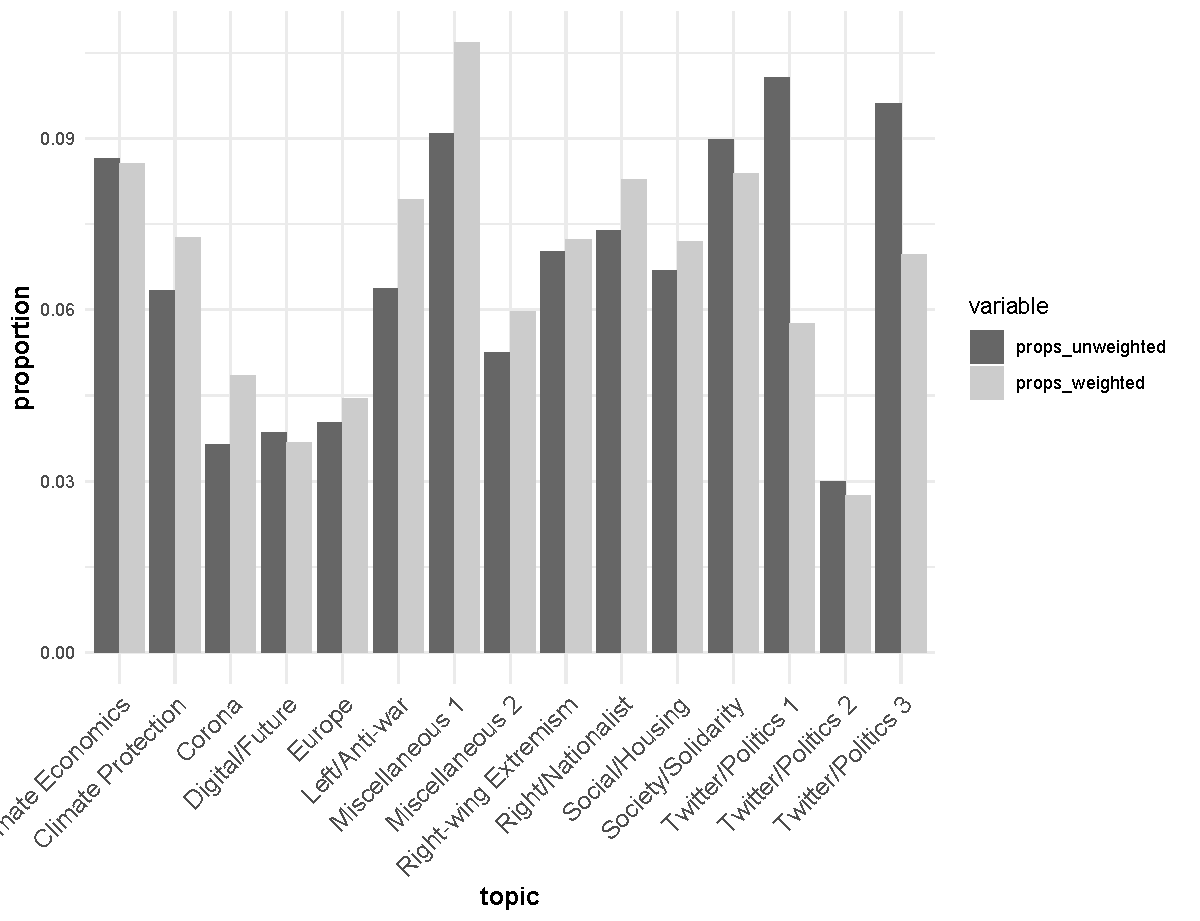
\includegraphics[scale = 0.40]{../plots/4_3/global_thetas.pdf}
	\end{figure}
\end{itemize}
\end{frame}

\begin{frame}
\frametitle{Model Selection and Global Characteristics}
\framesubtitle{Global Topic Correlations}
\begin{itemize}
\item Vocabulary overlap (left) and topic correlations (right):
\begin{figure}[h!]
  \resizebox{14cm}{!}{%	
  \centering
  \begin{subfigure}[b]{0.4\linewidth}
    \hspace*{-0.7cm}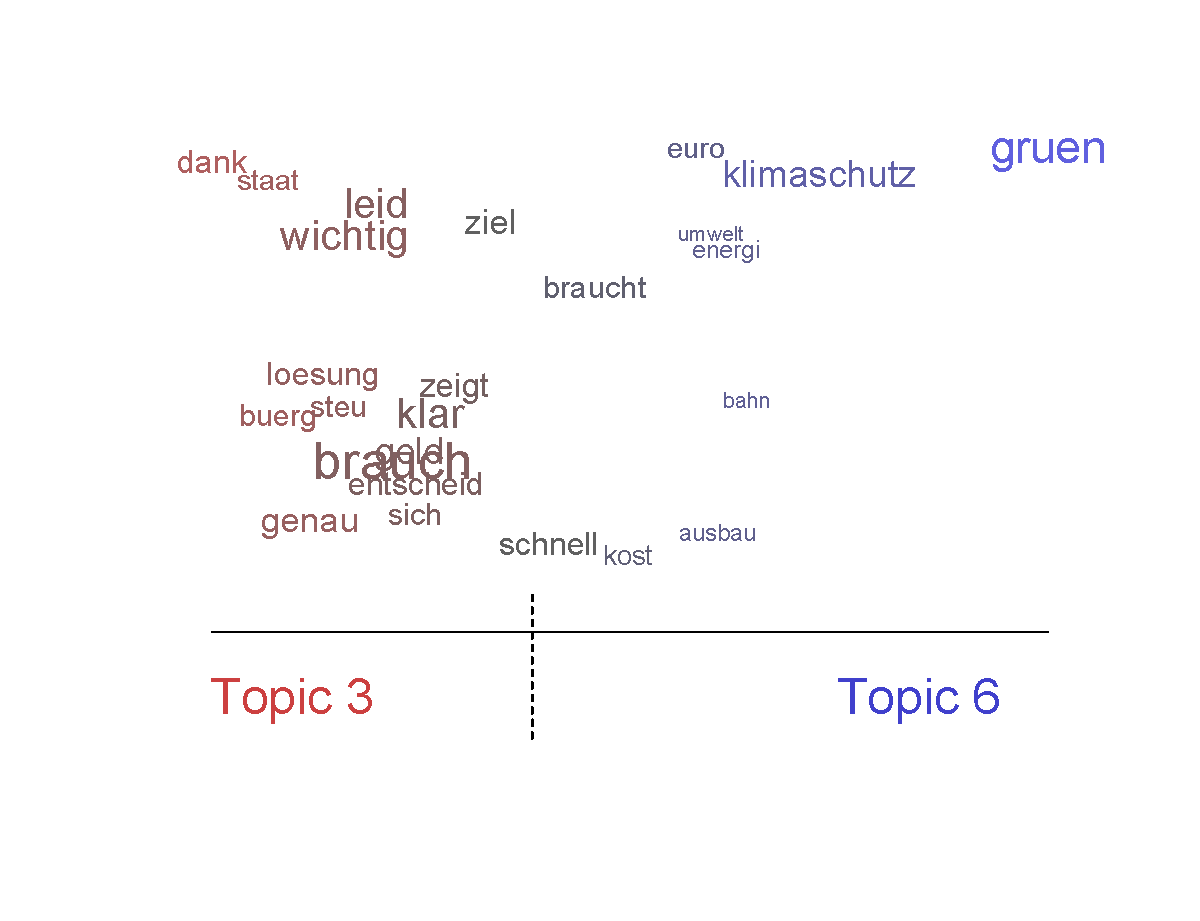
\includegraphics[width=\linewidth]{../plots/4_3/vocabulary_comparison.pdf}
  \end{subfigure}
  \begin{subfigure}[b]{0.4\linewidth}
    \hspace*{-1.1cm}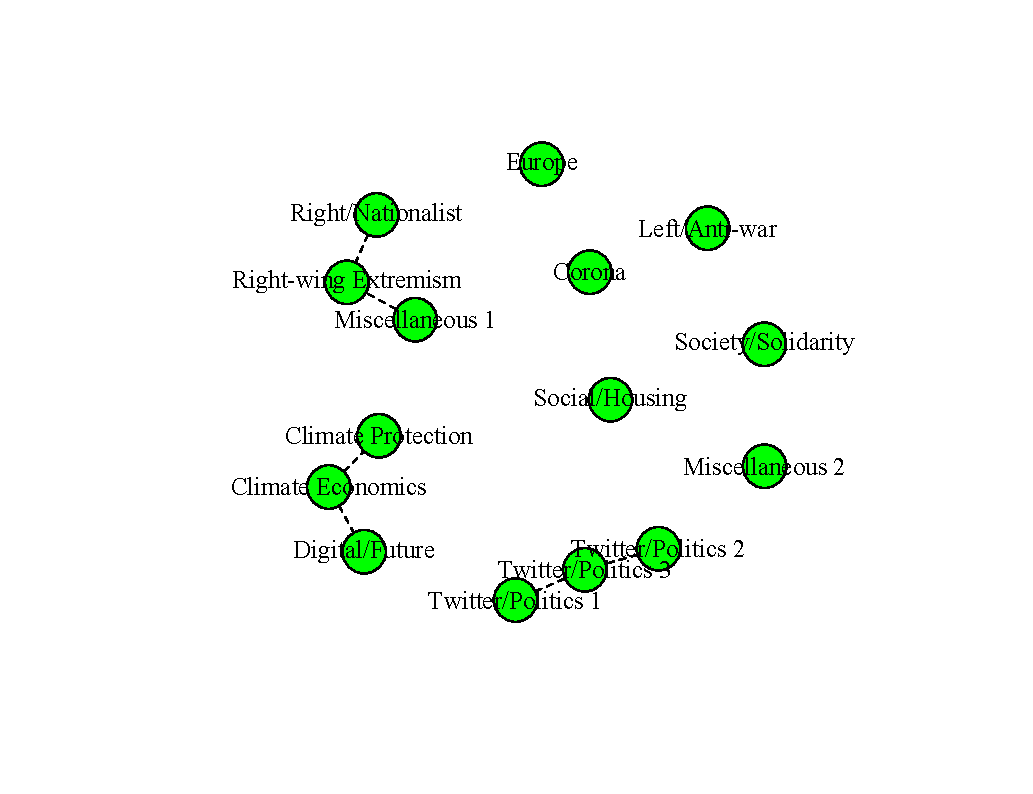
\includegraphics[width=\linewidth]{../plots/4_3/topic_correlations_map.pdf}
  \end{subfigure}
  }
\end{figure}		
\end{itemize}
\end{frame}

\begin{frame}
\frametitle{Bibliography}
\printbibliography
\end{frame}
\end{document}